\documentclass[aspectratio=169,xcolor=dvipsnames, t]{beamer}

\usepackage{cp24}
\usepackage{listings}
\usepackage{inconsolata}
\usepackage{bbding}
\usepackage{graphicx}        
\graphicspath{{images/}}

% Navigation oben anzeigen mit allen Sections
\setbeamertemplate{headline}[section in head/foot]
\setbeamercolor{section in head/foot}{bg=gray!15, fg=OliveGreen}
\setbeamercolor{section in head/foot shaded}{bg=gray!15, fg=OliveGreen!60!black}
\setbeamerfont{section in head/foot}{series=\bfseries}

%***
\title[Datenstrukturen und Entwurfsmethoden]{Datenstrukturen und Entwurfsmethoden}
\author[Ahmed Chtioui, Asma Mejbri, Mohamed Islem Slimane]{Ahmed Chtioui, Asma Mejbri, Mohamed Islem Slimane} 
\institute[]{

\includegraphics[scale=0.1]{logo.png}
}
\date[12.11.2025]{12.11.2025}
\beamertemplatenavigationsymbolsempty
\useinnertheme{rounded}
%***

\begin{document}

%===============================================================================
% Titelfolie
%===============================================================================
\begin{frame}
	\thispagestyle{empty}
	\titlepage
\end{frame}

%===============================================================================
% 1. Einführung
%===============================================================================
\section{Einführung}

\begin{frame}{Warum Datenstrukturen \& Algorithmen wichtig?}  
	\begin{itemize}
        \item  Grundlegende Bausteine jeder Software
        \vspace{0.3cm} 
        \item Schnellere und strukturiertere Programme \vspace{0.3cm}  
		\item Effiziente Verarbeitung großer Datenmengen 
        \vspace{0.3cm}  
		\item ermöglichen die Automatisierung von Aufgaben und Prozessen \vspace{0.3cm}  
        \item Häufig in Interviews vorkommend
        
	\end{itemize}
\end{frame}

%===============================================================================
% 2. Datenstrukturen
%===============================================================================
\section{Datenstrukturen}

\begin{frame}{Überblick über die Datenstrukturen und Entwurfsmethoden}
	\begin{columns}
		% Linke Spalte
		\begin{column}{0.45\textwidth}
			\textbf{\Large Lineare Datenstrukturen}
			\begin{itemize}
				\item Listen
				\item Arrays
				\item Stacks
			\end{itemize}

			\vspace{0.5cm}
			\textbf{\Large Nicht-lineare Strukturen}
			\begin{itemize}
				\item Hashing
                \item Heaps
			\end{itemize}
		\end{column}

		% Rechte Spalte
		\begin{column}{0.45\textwidth}
			\textbf{\Large Algorithmenentwurfsmethoden}
			\begin{itemize}
				\item Greedy
				\item Divide \& Conquer
				\item Brute-Force
				\item Backtracking
			\end{itemize}
		\end{column}
	\end{columns}
\end{frame}

%===============================================================================
% 3. Lineare Datenstrukturen
%===============================================================================
%===============================================================================
% 3. Lineare Datenstrukturen
%===============================================================================
\section{Lineare Datenstrukturen}

%---------------------------------------------------------------
% Listen – Definition
%---------------------------------------------------------------
\begin{frame}{Listen}

    \begin{block}{Definition}
Reihe von Elementen, die durch Verweise miteinander verbunden sind.    \end{block}

    \vspace{1em}

    \textbf{Merkmale}
    \begin{itemize}
        \item Dynamische Speicherverwaltung
        \item Zugriff erfolgt über Zeiger oder Referenzen
        \item Kein direkter Zugriff über Index
    \end{itemize}

\end{frame}
\begin{frame}{1. Verkettete Liste}

\begin{block}{Definition}
Eine Liste, bei der jeder Knoten auf den nächsten zeigt.
\end{block}

\vspace{1em}

\centering
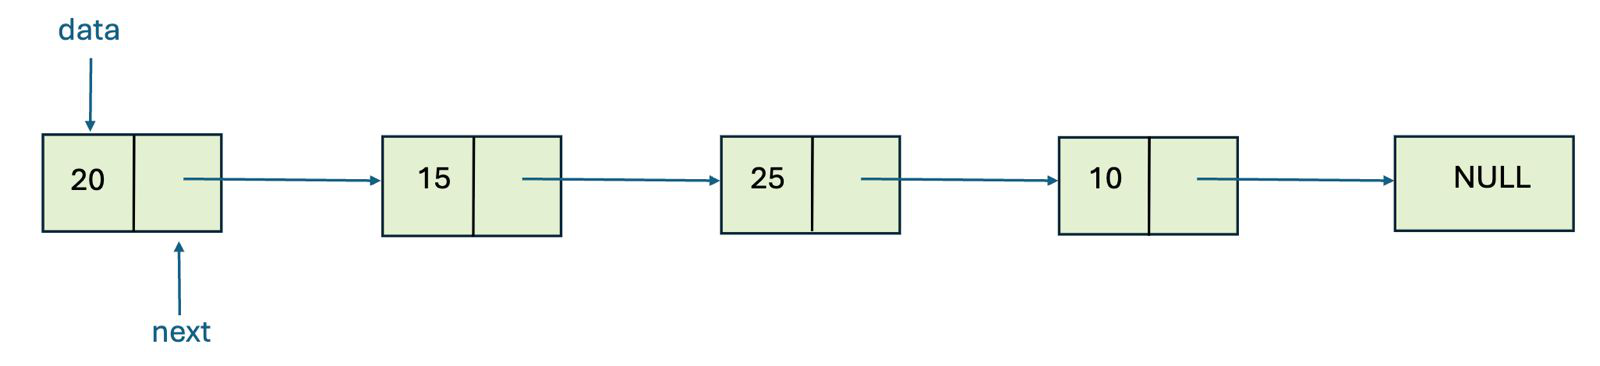
\includegraphics[width=0.9\textwidth]{list1.png}

\vspace{1em}

\raggedright
\textbf{Merkmale:}
\begin{itemize}
    \item Lineare Verbindung der Elemente
    \item Bewegung nur in eine Richtung

\end{itemize}

\end{frame}


\begin{frame}{2. Doppelt verkettete Liste}

\begin{block}{Definition}
Eine Liste, bei der jeder Knoten auf den vorherigen und den nächsten zeigt.
\end{block}

\vspace{1em}

\centering
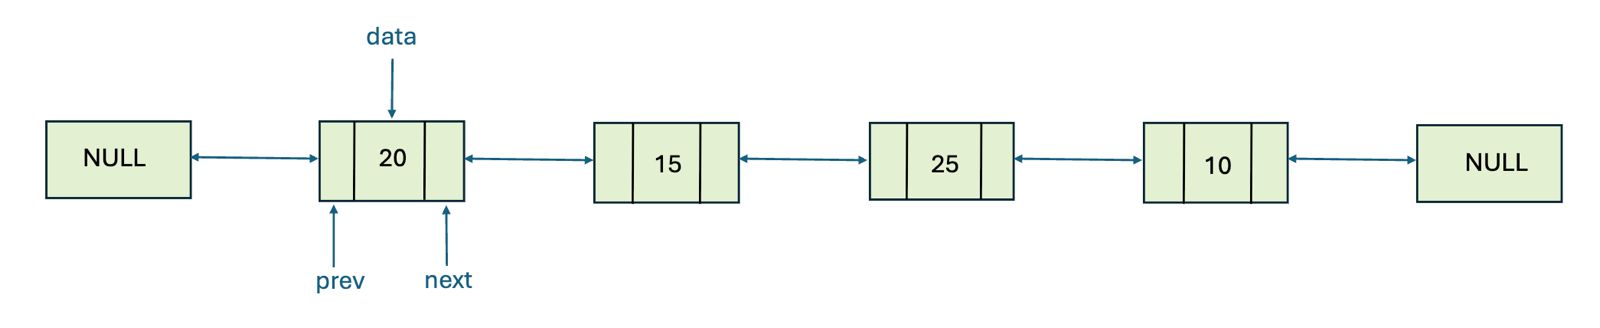
\includegraphics[width=0.9\textwidth]{list2.png}

\vspace{1em} % <-- vorher war 1.5em, jetzt kleiner für besseren Abstand

\begin{flushleft}
\textbf{Merkmale:}
\begin{itemize}
    \item Bewegung in beide Richtungen möglich (praktischer)
    \item Mehr Speicherbedarf wegen zwei Zeigern
\end{itemize}
\end{flushleft}

\end{frame}

\begin{frame}{3. Zirkuläre Liste}

\begin{block}{Definition}
Eine Liste, bei der der letzte Knoten wieder auf den ersten zeigt.
\end{block}

\vspace{1em}

\centering
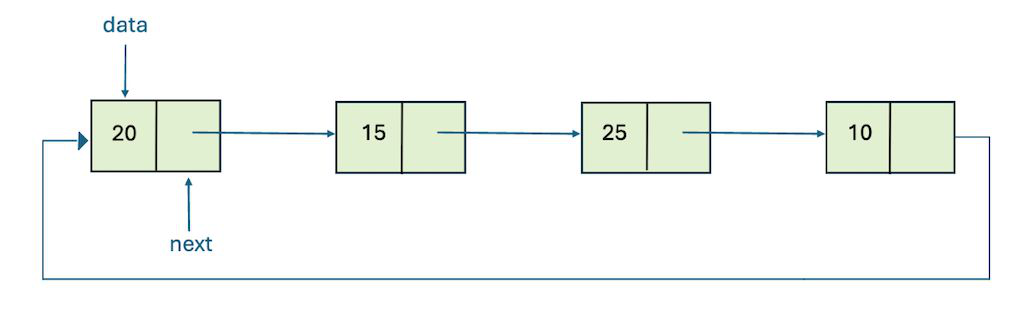
\includegraphics[width=0.7\textwidth]{list3.png} % vorher 0.9 -> jetzt kleiner

\vspace{1em}

\begin{flushleft}
\textbf{Merkmale:}
\begin{itemize}
    \item Ermöglicht endloses Durchlaufen der Liste
    \item Praktisch für zyklische Warteschlangen
\end{itemize}
\end{flushleft}

\end{frame}

\begin{frame}{Vergleich der Listenarten}

\centering
\textbf{Laufzeiten der wichtigsten Operationen}

\vspace{0.5cm}

\renewcommand{\arraystretch}{1.3}
\begin{tabular}{lccc}
\textbf{Operation} & \textbf{Verkettete Liste} & \textbf{Doppelt verkettete Liste} & \textbf{Zirkuläre Liste} \\
\hline
Einfügen am Anfang & O(1) & O(1) & O(1) \\
Einfügen am Ende & O(n) & O(1) & O(1) \\
Einfügen an Position & O(n) & O(n) & O(n) \\
Suche & O(n) & O(n) & O(n) \\
Löschen am Anfang & O(1) & O(1) & O(1) \\
Löschen am Ende & O(n) & O(1) & O(1) \\
Löschen an Position & O(n) & O(n) & O(n) \\
\end{tabular}

\end{frame}




\begin{frame}{Arrays}

    \begin{block}{Definition}
        Sammlung von Elementen gleichen Typs in zusammenhängenden Speicherbereichen.
    \end{block}

    \vspace{1em}

    \textbf{Merkmale}
    \begin{itemize}
        \item Lineare Anordnung
        \item Homogener Datentyp
        \item Einfache Iteration
        \item Direkter Zugriff 
    \end{itemize}
    

\end{frame}
\begin{frame}{Wie funktioniert ein Array?}
    \centering
    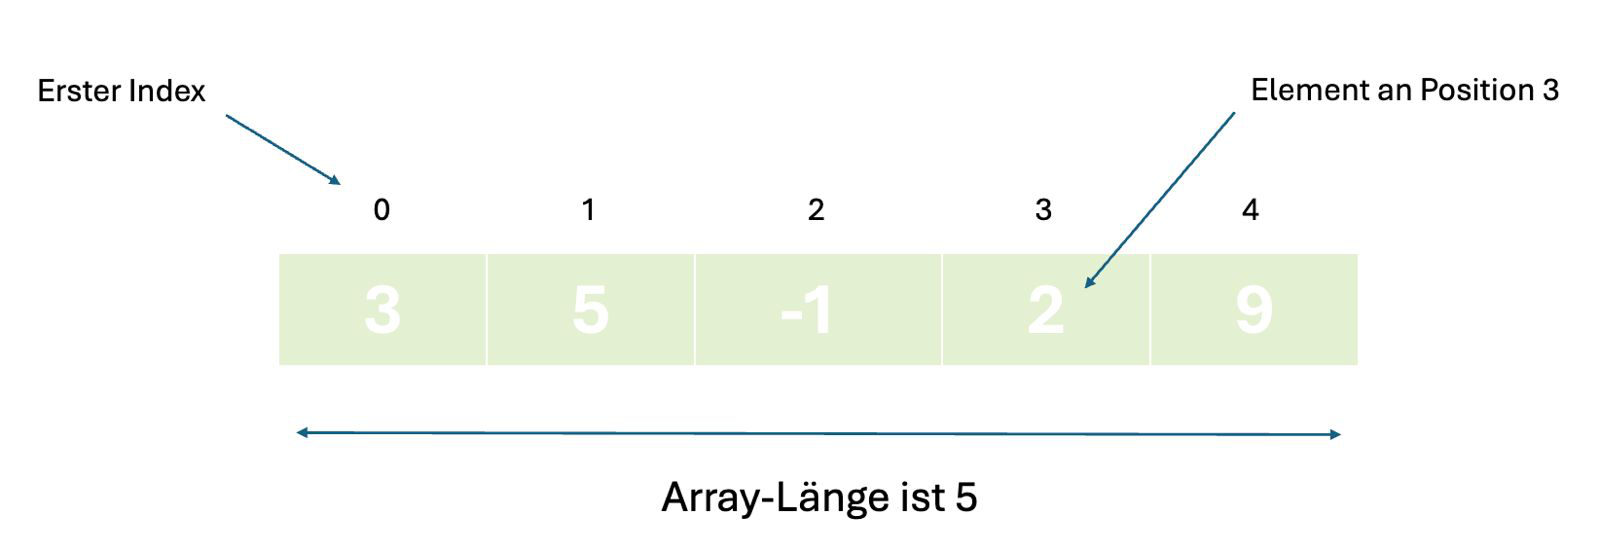
\includegraphics[width=0.8\textwidth]{example1.png}

    \vspace{1em}
    \textbf{Beispiel eines Arrays}

    \begin{itemize}
        \item Jedes Feld repräsentiert ein Element im Speicher  
        \item Zugriff über Index (z.\,B. \texttt{array[2]})  
    \end{itemize}
\end{frame}


%---------------------------------------------------------------
% Arrays – Typen 
%---------------------------------------------------------------
\begin{frame}{Arraytypen}

\textbf{Zwei Haupttypen von Arrays:}

\vspace{0.5cm}

\textbf{1. Statische Arrays}
\begin{itemize}
    \renewcommand{\labelitemi}{--}
    \item Feste Größe 
    \item Einfache Speicherverwaltung
    \item Unflexibel bei unbekannter Datenmenge
\end{itemize}

\vspace{0.4cm}

\textbf{2. Dynamische Arrays}
\begin{itemize}
    \renewcommand{\labelitemi}{--}
    \item Größe zur Laufzeit anpassbar
    \item Flexibler Speichergebrauch
    \item Manuelle Freigabe erforderlich
\end{itemize}

\end{frame}
\begin{frame}{Laufzeit von Arrays}

\centering
\textbf{Laufzeiten der wichtigsten Operationen}

\vspace{0.5cm}

\renewcommand{\arraystretch}{1.3}
\resizebox{0.95\textwidth}{!}{%
\begin{tabular}{lcc}
\textbf{Operation} & \textbf{Statisches Array} & \textbf{Dynamisches Array} \\
\hline
Zugriff auf Element  & O(1) & O(1) \\
Einfügen am Ende            & O(n) & O(1) \\
Einfügen an Position        & O(n) & O(n) \\
Löschen am Ende             & O(n) & O(1) \\
Löschen an Position         & O(n) & O(n) \\
Suche            & O(n) & O(n) \\
\end{tabular}
}
\end{frame}






%---------------------------------------------------------------
% Stacks – Konzept
%---------------------------------------------------------------
\begin{frame}{Stacks}

\begin{block}{Definition}
Datenstruktur, bei der Elemente  oben hinzugefügt und entfernt werden.( LIFO: last In, First Out).
\end{block}

\vspace{1em}

\textbf{Merkmale:}
\begin{itemize}
    \item Zugriff nur auf das oberste Element möglich
    \item Wichtige Operationen: \texttt{push}, \texttt{pop}
    \item Beispiel: Bücherstapel : das oberste Buch wird zuerst entfernt
\end{itemize}

\vspace{1em}

\centering
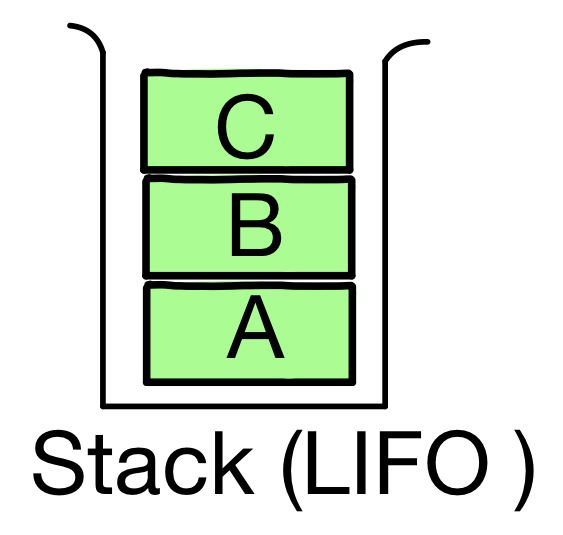
\includegraphics[width=0.1\textwidth]{stack_concept.jpg}

\end{frame}

%---------------------------------------------------------------
% Stacks – Operationen
%---------------------------------------------------------------
\begin{frame}{Operationen}

\begin{block}{Hauptoperationen}
\begin{itemize}
    \item \textbf{push(x)} : Fügt ein neues Element \texttt{x} oben auf den Stack.
    \item \textbf{pop()} : Entfernt das oberste Element und gibt es zurück.
\end{itemize}
\end{block}

\vspace{1em}

\begin{block}{Beispiel}
Angenommen, der Stack enthält [A, B] (B ist oben):
\begin{itemize}
    \item \texttt{push(C)} $\Rightarrow$ [A, B, C]
    \item \texttt{pop()} $\Rightarrow$ [A, B]
\end{itemize}
\end{block}

\vspace{1em}
\centering
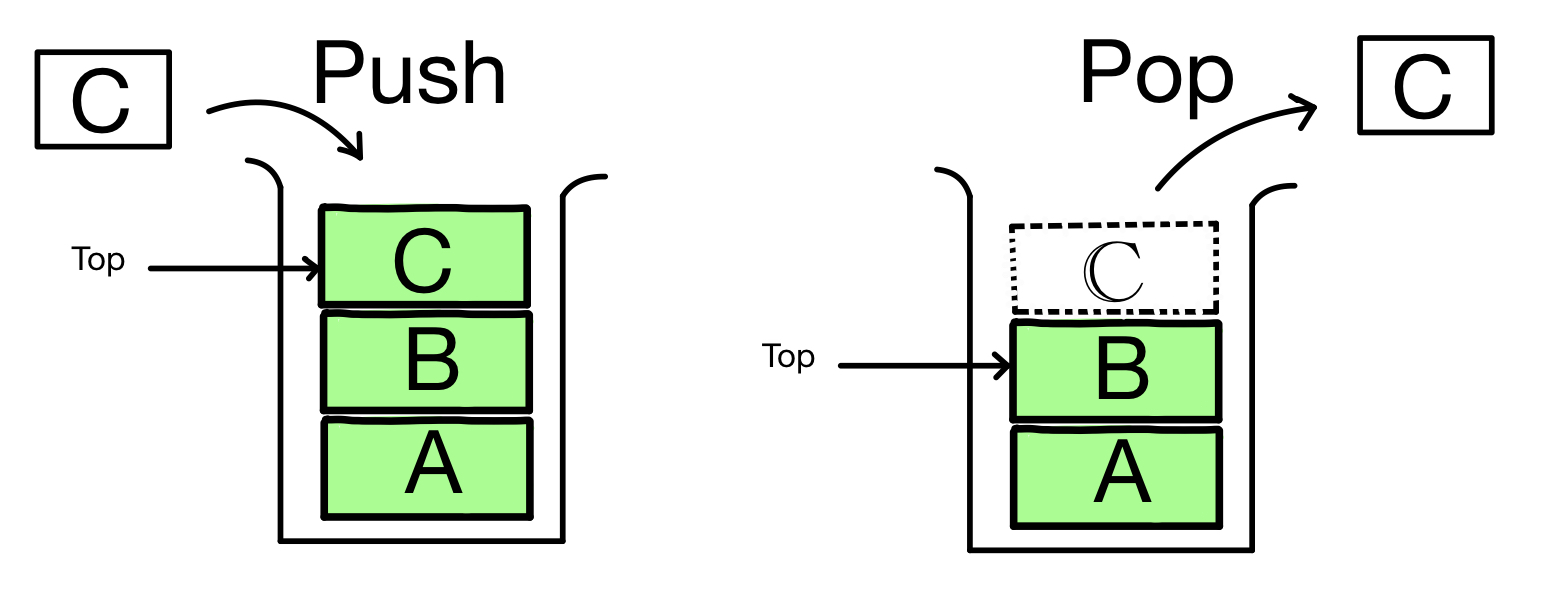
\includegraphics[width=0.3\textwidth]{stack_operations.jpg}

\end{frame}

\begin{frame}{Anwendung von Stacks}

\begin{block}{Beispiel: Rückgängig-Funktion (Undo)}
Ein Stack kann genutzt werden, um Aktionen rückgängig zu machen.
\end{block}

\vspace{0.5em}

\textbf{Ablauf:}
\begin{itemize}
    \item Aktionen werden nacheinander auf den Stack gelegt (\texttt{push})
    \item Beim Rückgängig-Machen wird die letzte Aktion entfernt (\texttt{pop})
\end{itemize}

\vspace{1em}
\centering
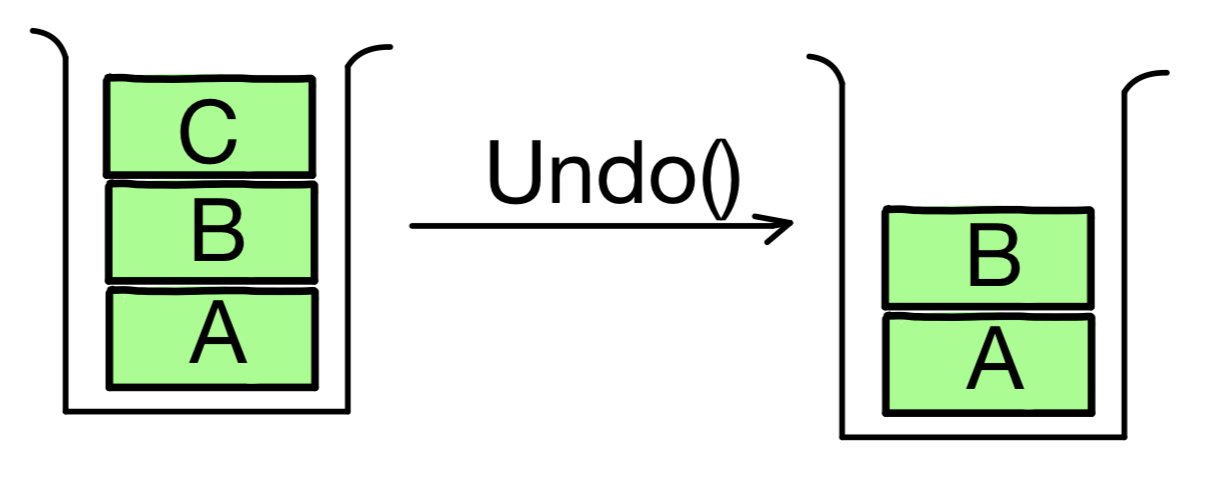
\includegraphics[width=0.5\textwidth]{stack_undo.jpg}

\end{frame}

%===============================================================================



%===============================================================================
% 4. Nicht-Lineare Datenstrukturen
%===============================================================================
\section{Nicht-Lineare Datenstrukturen}

% (später hinzufügen)

%===============================================================================
% Hashing – Teil 1: Einführung
%===============================================================================

\begin{frame}{Hashing}

\begin{block}{Definition}
Ein Verfahren, bei dem eine Eingabe beliebiger Länge 
mit Hilfe einer bestimmten mathematischen Funktion
in einen Wert fester Länge (\textbf{Hashwert}) umgewandelt wird.
\end{block}

\vspace{0.8em}

\textbf{Beispiel:}

\begin{itemize}
    \item \textbf{Hash-Funktion:} 
    \[
    f(x) = (\text{Summe der Buchstabenpositionen im Alphabet}) \mod 7
    \]
    
    \item \textbf{Berechnung:}
    \[
    f(\text{„Mike“}) = (M + i + k + e) = (13 + 9 + 11 + 5) = 38
    \]
    
    \item \textbf{Ergebnis:}
    \[
    38 \mod 7 = 3 \Rightarrow f(\text{„Mike“}) = 3
    \]
\end{itemize}


\end{frame}
\begin{frame}{Hashfunktionen in der Praxis}

\textbf{Anwendungen:}
\begin{itemize}
    \item Datenbanken
    \item Passwortspeicherung
    \item Kryptographie \& Blockchain (z.\,B. SHA-256)
\end{itemize}

\vspace{0.8em}

\textbf{Vorteile:}
\begin{itemize}
    \item[+] Konstante Zugriffszeit: O(1)
    \item[+] Effizient bei großen Datenmengen
\end{itemize}

\vspace{0.8em}

\textbf{Nachteile:}
\begin{itemize}
    \item[-] Kein sortierter Zugriff
    \item[-] Abhängig von der Hashfunktion
\end{itemize}

\end{frame}
\begin{frame}{Eigenschaften von Hashfunktionen}

\setlength{\itemsep}{1.8em} % more space between main points
\setlength{\parskip}{0.4em} % soft line spacing inside each point

\begin{itemize}
    \item \textbf{Deterministisch:}  
    Gleicher Input ergibt denselben Hashwert  
    
    \vspace{0.6em}
    \textit{Beispiel:} Hash("Mike") = 3, Hash("Mike") = 3

    \vspace{0.6em}
    \item \textbf{Kollisionsfrei:}  
    Unterschiedliche Eingaben haben verschiedene Hashwerte  
    
    \vspace{0.6em}
    \textit{Beispiel:} Hash("Mike") = 11, Hash("John") = 11 \textcolor{red}{\textbf{X}}

    \vspace{0.6em}
    \item \textbf{Avalanche-Effekt:}  
    Kleine Änderungen im Input erzeugen stark unterschiedliche Hashwerte  
    
    \vspace{0.6em}
    \textit{Beispiel:} Hash("Mike") = 1230, Hash("Mika") = 246

    \vspace{0.6em}
    \item \textbf{Irreversibel:}  
    Aus dem Output kann der ursprüngliche Input nicht gefunden werden  
    
    \vspace{0.6em}
    \textit{Beispiel:} Hash(unbekannt) = 15
\end{itemize}

\end{frame}

% Heaps
%===============================================================================

\begin{frame}{Heap – Definition \& Eigenschaften}
\begin{block}{Definition}
 eine baumbasierte Datenstruktur, die die \textbf{Heap-Eigenschaft} erfüllt:
\begin{itemize}
    \item \textbf{Max-Heap:} Jeder Elternknoten ist größer oder gleich seinen Kindern
    \item \textbf{Min-Heap:} Jeder Elternknoten ist kleiner oder gleich seinen Kindern
\end{itemize}
\end{block}

\vspace{0.5em}
\textbf{Eigenschaften:}
\begin{itemize}
    \item ein vollständiger binärer Baum
    \item typischerweise in einem Array gespeichert:
    \[
\text{left}(i) = 2i,\quad 
\text{right}(i) = 2i + 1,\quad 
\text{parent}(i) = \left\lfloor \frac{i}{2} \right\rfloor
\]

     \\
    z.\,B. \(i=1\) ist die Wurzel, \(i=2\) und \(i=3\) sind ihre Kinder usw.  
  
\end{itemize}
\end{frame}

%===============================================================================
% Beispiel Max-Heap
%===============================================================================
\begin{frame}{Beispiel: Max-Heap}

% Abstand zwischen Titel und Bild (hier anpassbar)
\vspace{0.3cm} % <-- ändere diesen Wert, z.B. 0.2cm, 1cm oder 2cm

% Bild (zentriert, aber kann leicht angepasst werden)
\begin{center}
    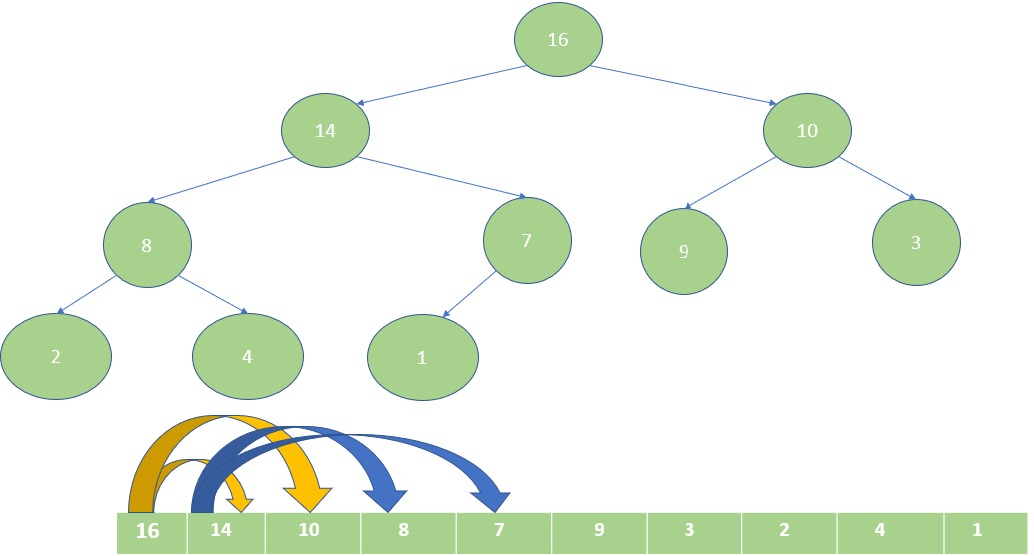
\includegraphics[width=0.7\textwidth]{pic11.png}
\end{center}

% Optional: zusätzlicher Abstand nach unten (falls du das Bild höher oder tiefer willst)
\vspace{0.3cm} % <-- ebenfalls anpassbar oder entfernen

\end{frame}



\begin{frame}{Wichtige Operationen}

\small
\renewcommand{\arraystretch}{1.5}

\begin{center}
\begin{tabular}{p{3cm} p{8.5cm} p{2.3cm}}
\textbf{Operation} & \textbf{Beschreibung} & \textbf{Laufzeit} \\ \hline

\textbf{insert(heap,x)} &
Neues Element einfügen dann Ordnung durch \textbf{heapifyUp} wiederherstellen. &
$\mathcal{O}(\log n)$ \\[4pt]

\textbf{extract(heap)} &
Wurzel entfernen dann Ordnung durch \textbf{heapifyDown} &
$\mathcal{O}(\log n)$ \\[4pt]

\textbf{peek(heap)} &
Wurzel ausgeben ohne sie zu entfernen. &
$\mathcal{O}(1)$ \\[4pt]

\textbf{heapifyUp(heap,i)} &
Nach \textbf{insert}: Element steigt nach oben, solange größer(Max-Heap) / kleiner (Min-Heap) als Elternknoten. &
$\mathcal{O}(\log n)$ \\[4pt]

\textbf{heapifyDown(heap,i)} &
Nach \textbf{extract}: Wurzel sinkt nach unten, bis größer(Max-Heap) / kleiner(Min-Heap) als beide Kinder. &
$\mathcal{O}(\log n)$ \\

\end{tabular}
\end{center}
\end{frame}

%===============================================================================
% Beispiel 1: Insert (Max-Heap)
%===============================================================================
\begin{frame}{Beispiel: Insert beim Max-Heap}
\small
\begin{columns}[T,onlytextwidth]

    %--- Linke Spalte: Text ---
    \begin{column}{0.52\textwidth}
        \textbf{Schritte:}
        \begin{itemize}
            \item Füge \texttt{50} am Ende ein → \texttt{[40, 30, 10, 5, 50]}
            \item Vergleiche mit Eltern (\texttt{30}): 50 $>$ 30 $\rightarrow$ tauschen
            \item Vergleiche mit nächstem Eltern (\texttt{40}): 50 $>$ 40 $\rightarrow$ tauschen
        \end{itemize}
    \end{column}

    %--- Rechte Spalte: Bild ---
    \begin{column}{0.46\textwidth}
        \centering
        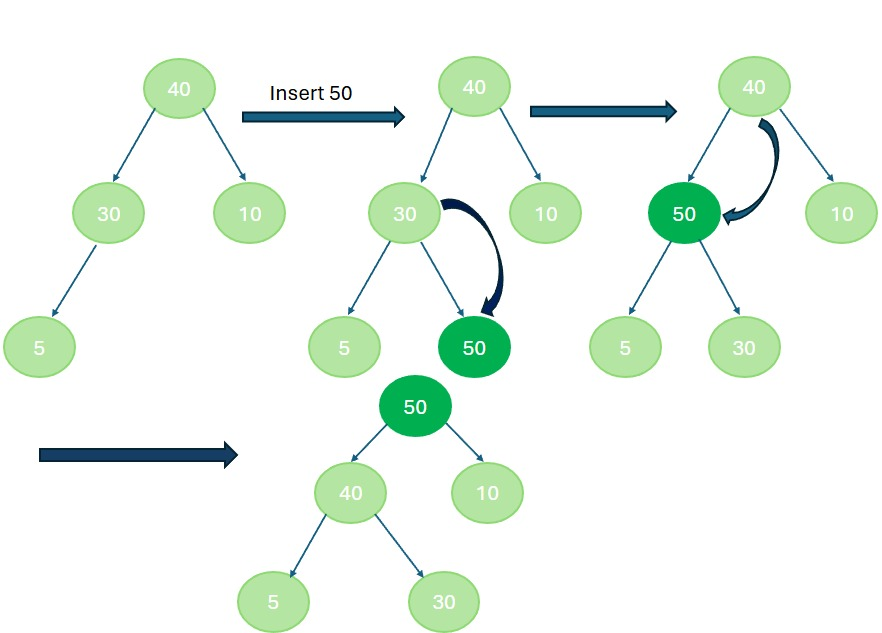
\includegraphics[width=1\textwidth]{insert.png}
    \end{column}

\end{columns}
\end{frame}

%===============================================================================
% Beispiel 2: Extract (Max-Heap)
%===============================================================================
\begin{frame}{Beispiel: Extract beim Max-Heap}
\small
\begin{columns}[T,onlytextwidth]

    %--- Linke Spalte: Bild ---
    \begin{column}{0.52\textwidth}
        \textbf{Schritte:}
        \begin{itemize}
            \item Entferne Wurzel (12) → letztes Element (9) nach oben
            \item Vergleiche mit Kindern (6, 10): 10 ist größer $\rightarrow$ tauschen
            \item Vergleiche erneut: 9 $>$ 5 $\rightarrow$ Heap korrekt
        \end{itemize}
    \end{column}


    %--- Rechte Spalte: Text ---
    \begin{column}{0.46\textwidth}
        \centering
        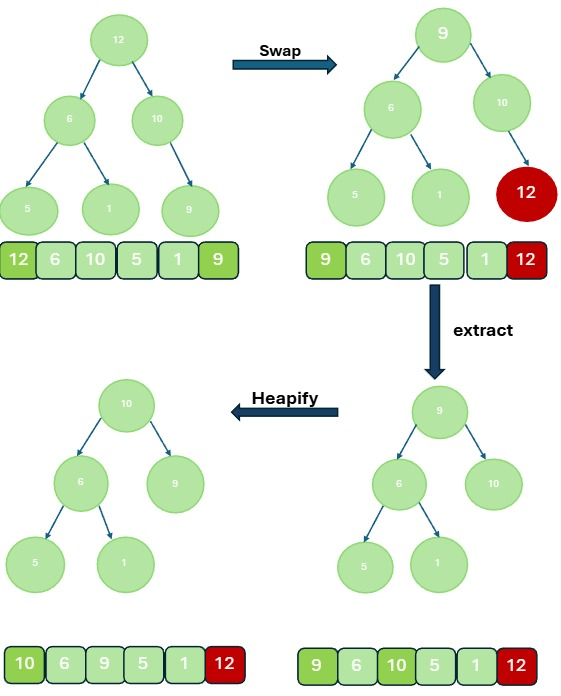
\includegraphics[width=0.8\textwidth]{extract.png}
    \end{column}


\end{columns}
\end{frame}










\begin{frame}{Anwendungen von Heaps}
\begin{block}{Common Uses}
\begin{itemize}
    \item \textbf{Priority Queues:}  Verwaltung von Aufgaben nach Priorität
    \item \textbf{Heapsort:}  Sortieralgorithmus mit Laufzeit \(O(n \log n)\)
    \item \textbf{Dijkstra-Algorithmus:}  Kürzeste Wege in Graphen
    \item \textbf{Prim-Algorithmus:}  Minimaler Spannbaum
    \item \textbf{Scheduling-Systeme:}  Prozesse mit Priorität
\end{itemize}
\vspace{0.3cm}
\textit{spätere Vorträge dazu\dots}
\end{block}
\end{frame}

%===============================================================================
% 5. Algorithmenentwurfsmethoden
%===============================================================================




\section{Algorithmenentwurfsmethoden}


%---------------------------------------------------------------
% Greedy – Konzept
%---------------------------------------------------------------
\begin{frame}{Greedy}

\begin{block}{Definition}
Ein Verfahren, bei dem in jedem Schritt die lokal beste Entscheidung gewählt wird,
um am Ende die möglichst optimale Lösung zu erreichen.

\end{block}

\vspace{0.8em}

\textbf{Merkmale:}
\begin{itemize}
    \item Wählt stets die beste sofortige Option
    \item Keine Rückverfolgung (Backtracking)
    \item Einfach und schnell, aber nicht immer optimal
\end{itemize}
\end{frame}

%---------------------------------------------------------------
% Greedy – Ablauf
%---------------------------------------------------------------
\begin{frame}{Funktionseise}

\begin{block}{Allgemeiner Ablauf}
\begin{enumerate}
    \item Initialisiere Lösung (leer)
    \item Wiederhole, solange Elemente verfügbar sind:
    \begin{itemize}
        \item Wähle das \textbf{beste verbleibende Element}
        \item Füge es der Lösung hinzu
        \item Überprüfe, ob die Lösung gültig bleibt
    \end{itemize}
    \item Gib die gebildete Lösung zurück
\end{enumerate}
\end{block}



\end{frame}


%---------------------------------------------------------------
% Greedy – Beispiel: Münzwechselproblem (Schritt-für-Schritt)
%---------------------------------------------------------------
\begin{frame}{Beispiel: Münzwechselproblem}

\begin{block}{Problem}
\textbf{Gegeben:} Münzen mit den Werten 50, 20, 10, 5, 2, 1  
\\
\textbf{Gesucht:} Minimale Anzahl Münzen für einen Betrag.
\end{block}

\vspace{0.6em}

\textbf{Greedy-Schritte für Betrag = 76:}
\begin{enumerate}
    \item Starte mit Restbetrag = 76
    \item Wähle größte mögliche Münze:
    \begin{itemize}
        \item 76 – 50 = 26
        \item 26 – 20 = 6
        \item 6 – 5 = 1
        \item 1 – 1 = 0
    \end{itemize}
    \item Lösung: \textbf{4 Münzen (50, 20, 5, 1)}.
\end{enumerate}

\vspace{0.8em}
\centering
\textbf{Ergebnis:} \fbox{Minimal = 4 Münzen für Betrag 76}

\end{frame}



\begin{frame}{Divide \& Conquer}

\begin{block}{Definition}
Ein Ansatz, bei dem ein großes Problem in kleinere Teilprobleme geteilt wird,  
diese einzeln gelöst und schließlich zu einer Gesamtlösung kombiniert werden.
\end{block}

\vspace{1em}

\textbf{Funktionsweise:}
\begin{itemize}
    \item \textbf{Divide:} Das Problem wird in kleinere Teilprobleme zerlegt.
    \item \textbf{Conquer:} Die Teilprobleme werden rekursiv gelöst und kombiniert.
\end{itemize}

\vspace{1em}

\textbf{Vorteile:}
\begin{itemize}
    \item[\textcolor{green!60!black}{+}] Gute Laufzeit bei großen Problemen
    \item[\textcolor{green!60!black}{+}] Klare, strukturierte Vorgehensweise durch Rekursion
\end{itemize}

\textbf{Nachteile:}
\begin{itemize}
    \item[\textcolor{green!60!black}{-}] Zusätzlicher Speicherbedarf durch Rekursion
    \item[\textcolor{green!60!black}{-}] Rekursive Implementierung kann komplex sein
\end{itemize}

\end{frame}

\begin{frame}{Beispiel: Binary search}

\vspace{-0.8em} % moves everything up
\textbf{Ziel: finde die Zahl 7}

\vspace{-0.4em} % reduce space between text and image
\begin{center}
    \includegraphics[width=0.5\textwidth]{divide.png}
\end{center}

\end{frame}



\begin{frame}{Brute Force}

\begin{block}{Definition}
Ein Brute-Force-Algorithmus prüft \textbf{alle möglichen Lösungen}, 
bis die \textbf{richtige} gefunden ist.
\end{block}

\vspace{0.8em}

\textbf{Merkmale:}
\begin{itemize}
    \item Systematische Suche durch alle Möglichkeiten
    \item Garantiert eine korrekte Lösung (wenn vorhanden)
    \item Einfach zu verstehen und zu implementieren
    \item Sehr hohe Laufzeit für große Eingaben
\end{itemize}



\end{frame}


\begin{frame}{Funktionsweise}

\begin{block}{Allgemeiner Ablauf}
\begin{enumerate}
    \item Erzeuge alle möglichen Kandidatenlösungen
    \item Für jede Lösung:
    \begin{itemize}
        \item Überprüfe, ob sie gültig ist
        \item Bewerte ihre Qualität (z. B. Kosten, Länge, etc.)
    \end{itemize}
    \item Wähle die \textbf{beste gültige Lösung}
\end{enumerate}
\end{block}



\end{frame}


\begin{frame}{Beispiel :}


\vspace{0.8em}

\textbf{Passwortsuche:}

\begin{center}
\begin{tabular}{lcl}
\texttt{data} & $\rightarrow$ & \XSolidBrush\\
\texttt{struktur} & $\rightarrow$ & \XSolidBrush \\

\texttt{projekt} & $\rightarrow$ & \CheckmarkBold \textbf{Gefunden!}
\end{tabular}
\end{center}

\vspace{0.5em}

\textbf{In diesem Fall ist „projekt“ das Passwort.}

\vspace{0.5em}

\textit{Brute Force testet alle Kombinationen, bis die richtige gefunden ist.}

\end{frame}


\begin{frame}{Backtracking}

\begin{block}{Definition}
Eine Methode, bei der man eine Lösung schrittweise aufbaut, verschiedene Möglichkeiten ausprobiert und bei einem falschen Weg zurückgeht, um eine andere Option zu testen.
\end{block}

\vspace{0.5em}

\textbf{Merkmale:}
\begin{itemize}
    \item Arbeitet nach dem {„Versuch-und-Irrtum“-Prinzip (trial and error)}
    \item Baut eine Teillösung Schritt für Schritt auf
    \item Wenn eine Regel verletzt wird → \textbf{Rückkehr zum vorherigen Zustand}
    \item Wird häufig mit \textbf{Rekursion} implementiert
\end{itemize}

\end{frame}


\begin{frame}[fragile]{Funktionsweise}

\begin{block}{Pseudocode}
\lstset{
    literate={ä}{{\"a}}1 {ö}{{\"o}}1 {ü}{{\"u}}1
             {Ä}{{\"A}}1 {Ö}{{\"O}}1 {Ü}{{\"U}}1
             {ß}{{\ss}}1
}
\begin{lstlisting}[language=Python, basicstyle=\ttfamily\small]
Funktion FindeLösung(Stufe, Vektor):
    solange es noch Möglichkeiten gibt:
        wähle eine neue Möglichkeit
        falls gültig (z.B. keine Regel verletzt wird):
            füge sie zum Vektor hinzu  #Teil-Lösung erweitern
            falls vollständig:
                return True   #Lösung gefunden
            sonst:
                FindeLösung(Stufe+1, Vektor)
            mache letzte Wahl rückgängig  #Backtracking
    return False  #keine Lösung
\end{lstlisting}
\end{block}

\end{frame}


\begin{frame}{Beispiele:}

% Text nicht einrücken & linksbündig
\setlength{\parindent}{0pt}
\raggedright

% 1) Rucksackproblem
\begin{columns}[c,onlytextwidth]
  \begin{column}{0.18\textwidth}
    \centering
    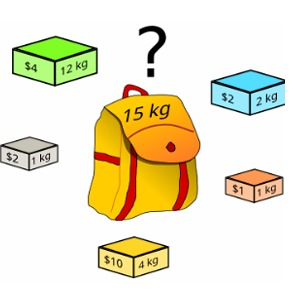
\includegraphics[width=0.8\linewidth]{knapsack.png}
  \end{column}
  \begin{column}{0.82\textwidth}
    \textbf{Rucksackproblem:} Wähle Gegenstände mit maximalem Wert, aber unterhalb einer Gewichtsgrenze.
  \end{column}
\end{columns}

\vspace{0.5em}

% 2) Sudoku
\begin{columns}[c,onlytextwidth]
  \begin{column}{0.18\textwidth}
    \centering
    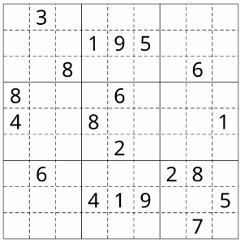
\includegraphics[width=0.8\linewidth]{sudoku.png}
  \end{column}
  \begin{column}{0.82\textwidth}
    \textbf{Sudoku:} Zahlen nach Regeln in ein Raster einfügen.
  \end{column}
\end{columns}

\vspace{0.5em}

% 3) Färbeproblem
\begin{columns}[c,onlytextwidth]
  \begin{column}{0.18\textwidth}
    \centering
    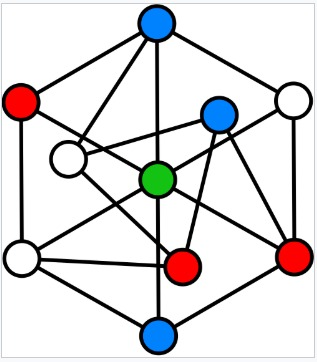
\includegraphics[width=0.8\linewidth]{graph-coloring.png}
  \end{column}
  \begin{column}{0.82\textwidth}
    \textbf{Färbeproblem:} Knoten so einfärben, dass Nachbarknoten unterschiedliche Farben haben.
  \end{column}
\end{columns}

\end{frame}

\begin{frame}{Laufzeit}

\begin{block}{Allgemein}
Bei \textbf{Backtracking} werden viele Möglichkeiten ausprobiert, 
bis eine gültige Lösung gefunden wird.  
Das kann problematisch sein, wenn es \textbf{viele Optionen} gibt.
\end{block}

\vspace{0.8em}

\textbf{Laufzeit im schlechtesten Fall:}
\[
O(z^N)
\]

\begin{itemize}
    \item \(z\) = Anzahl der \textbf{Möglichkeiten pro Schritt}
    \item \(N\) = Anzahl der \textbf{benötigten Schritte}
\end{itemize}

\vspace{0.8em}

\textbf{Beispiel:}  
Wenn es 7 Ebenen gibt und pro Stufe 4 Möglichkeiten bestehen:
\[
4^7 = 16{,}384 \text{ mögliche Versuche}
\]

\vspace{0.5em}
\textcolor{red!70!black}{\textbf{→ Fazit:}} Die Laufzeit kann \textbf{exponentiell wachsen}!

\end{frame}

\begin{frame}{Feedback}

\begin{block}{Bewertung des Backtracking-Algorithmus}
\begin{itemize}
    \item \textbf{Zuverlässig:} Findet immer eine Lösung, wenn eine existiert.  
    \item \textbf{Nicht effizient:} sehr langsam, wenn es viele Möglichkeiten gibt.  
    \item \textbf{Praktisch:} Gut geeignet für kleine Probleme
\end{itemize}
\end{block}

\vspace{0.8em}

\textcolor{OliveGreen!80!black}{\textbf{Fazit:}}  
Backtracking ist sicher, aber nicht ideal , wenn man lieber eine garantierte Lösung als maximale Effizienz möchte.

\end{frame}


%===============================================================================
% Problem (allgemein)
%===============================================================================
\begin{frame}{Problem}

\begin{block}{Aufgabenstellung}
Gegeben ist ein unsortiertes Array mit \(n > 5\) Zahlen.

\textbf{Ziel:} Sortiere das Array in aufsteigender Reihenfolge.
\end{block}

\vspace{0.5cm}

\textbf{Herausforderung:}
\begin{itemize}
    \item Das Array ist zu groß, um jedes Element manuell zu vergleichen
    \item Direkte Sortierverfahren wie Bubble Sort sind ineffizient bei größeren Arrays
    \item Man möchte die Anzahl der Vergleiche und Verschiebungen minimieren
\end{itemize}

\vspace{0.5cm}

\textbf{Frage an den Leser:} Wie könnte man das Problem effizient lösen, indem man das Array in kleinere Teilprobleme zerlegt und anschließend die Teillösungen kombiniert?

\end{frame}



%===============================================================================
% Pseudocode Slide – Divide & Conquer Sort
%===============================================================================
\begin{frame}[fragile]{Lösung}

\begin{block}{Pseudocode}
\lstset{
    literate={ä}{{\"a}}1 {ö}{{\"o}}1 {ü}{{\"u}}1
             {Ä}{{\"A}}1 {Ö}{{\"O}}1 {Ü}{{\"U}}1
             {ß}{{\ss}}1
}
\begin{lstlisting}[language=Python, basicstyle=\ttfamily\small]
Funktion DivideAndConquerSort(A):
    falls Länge(A) <= 1:
        return A  # Array ist bereits sortiert
    # 1. Teile das Array in zwei Hälften
    mid = Länge(A) // 2
    left  = A[0 : mid]
    right = A[mid : end]
    # 2. Sortiere beide Hälften rekursiv
    leftSorted  = DivideAndConquerSort(left)
    rightSorted = DivideAndConquerSort(right)
    # 3. Führe die sortierten Hälften zusammen
    return merge(leftSorted, rightSorted)
\end{lstlisting}
\end{block}

\end{frame}

%===============================================================================
% Beispiel: Konkretes Array
%===============================================================================
\begin{frame}{Beispiel:}

\begin{block}{Konkretes Array}
Für das folgende Array soll die Sortierung demonstriert werden:

\[
\texttt{array = [79, 15, 10, 43, 2, 8, 35, 26]}
\]
\end{block}

\begin{center}
    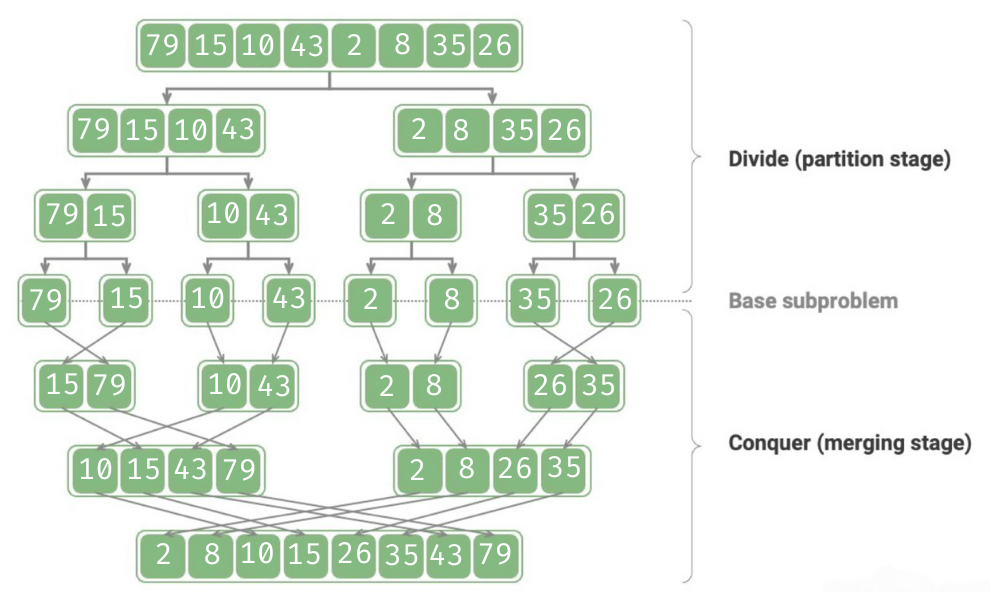
\includegraphics[width=0.5\linewidth]{problem.png}
\end{center}

\end{frame}


%===============================================================================
% 6. Zusammenfassung
%===============================================================================
\begin{frame}{Zusammenfassung}

\begin{itemize}
    \item Verstehen des Problemtyps
    \item Analyse von Zeit- und Speicherkomplexität
    \item Analyse der positiven und negativen Eigenschaften
    \item Beachten der Datenänderung und -größe
\end{itemize}

\vspace{0.6cm}
\begin{center}
$\Rightarrow$ \textbf{Die zur Aufgabe passende Datenstruktur und der richtige Algorithmus sind für eine effiziente Problemlösung entscheidend.}
\end{center}
\vspace{0.5cm}
\begin{block}{Fragen?}
Vielen Dank für Ihre Aufmerksamkeit!
\end{block}



\end{frame}

\end{document}